\documentclass[twocolumn,11pt]{article}
\usepackage{usenix}
\usepackage{url}
\usepackage{graphics}
\usepackage{hyperref}
\usepackage{epsfig}
\usepackage{listings}
\usepackage{color}
\lstset{language=C}
\lstset{
    basicstyle=\ttfamily\small,
    keywordstyle=\color{blue},
    commentstyle=\color{green}
}
\newcommand{\chumma}[1]{\subsubsection {#1}}
\newcommand{\mus}{$\mu s$}
\setlength{\parindent}{0in}

% -------------------------------------------------------------------------
%                                   Title
% -------------------------------------------------------------------------

\title{\bf \textsf{Measurement of certain File System parameters}}

\author{Priyananda Shenoy\
\\
       {\em \normalsize Department of Computer Sciences}\\
       {\em \normalsize University of Wisconsin, Madison, WI}\\
       {\tt \normalsize shenoy@cs.wisc.edu}}

\begin{document}
\date{}
\raggedbottom

\maketitle

\pagenumbering{arabic}
\pagestyle{plain}
\setlength{\footskip}{25pt}

% -------------------------------------------------------------------------
%                               Introduction
% -------------------------------------------------------------------------
\begin{abstract}
\small
Careful measurement of file system parameters is of utmost importance in
evaluating how well a system is performing. This paper describes some ideas
and methodologies for measuring a few important file system parameters, namely:
the ideal buffer size for random reads, the amount of prefetching during
sequential reads, the size of the system file cache and the number of direct
blocks accessible through the inode. We also analyze the results of running
these measurements on a test system, and interpret the results.
\end{abstract}

\begin{sloppypar}

% -------------------------------------------------------------------------
%                               Introduction
% -------------------------------------------------------------------------
\section{Introduction}
\label{sec:Introduction}

\noindent Since file systems form the core of most operating systems, the
performance of the file system has a significant impact on the overall
performance of the system. Therefore accurate measurements of different
characteristics of the file system are often needed. In this paper, we
analyze in detail the approaches, methodologies and issues related
to measuring certain file system parameters. The questions which we tackle
in this paper are:
\begin{itemize}
	\item What is the ideal buffer size for random reads?
	\item How much data is prefetched when a file is being read sequentially?
	\item How large is the system file cache?
	\item How many blocks are directly accessible from the inode, without
		another level of indirection?
\end{itemize}
We explore each of these questions in detail. We also present the results of
running our tests on a test system, and compare the outcome against our
expected outcome.

\subsection{Organization of the paper}
\noindent Section 2 describes the methodology behind our measurements. 
Section 3 describes the specifications of test system. Section 4 describes
the implementation and results of the measurements. Section 5 summarizes
the conclusions obtained from the tests.

% -------------------------------------------------------------------------
%                              Methodology
% -------------------------------------------------------------------------
\section{Methodology}
\label{sec:Methodology}

\subsection{Timers}

Every measurement is as good as the timer used to make that measurement.
For measuring time accurately, we used the {\tt RDTSC} instruction
provided by the x86 architecture \cite{wiki_rdtsc}. This
instruction gives us the smallest granularity possible on the system,
which is equal to the duration of one clock cycle. However
the following caveats have to be considered while using this
instruction:
\begin{enumerate}
	\item On a multi-core system, this instruction is not guaranteed to
	return the same value on all cores, so values obtained on different
	cores are not comparable. We get around this issue by forcing our
	process to run on one of the cores via the {\tt sched\_setaffinity}
	system call \cite{sched_affinity}.
	\item Most modern processors dynamically change the clock frequency
	depending on load, which would invalidate our measurements. We avoid
	this issue by turning off the power-saving features of the processor
	for the duration of the tests.
\end{enumerate}

\subsection{Ideal buffer size for random access}

Random access to any part of the file is accomplished by seeking to the
desire location using {\tt lseek}, and then reading data from that location.
Since the smallest unit of transfer for the file system is the \textit{block},
any request to read data smaller than a block will still cause the system to
read an entire block. Hence the ideal amount to read in a single random read is
equal to the size of the block.

This picture is complicated by the \textit{prefetching} behavior of modern 
file systems. When the system detects that the file is being read in a 
sequential manner, the system automatically reads the next few blocks of the
file in anticipation of further reads. Fortunately the POSIX standard provides
the function {\tt posix\_fadvice} \cite{posix_fadvise}, which allows us to turn off 
prefetching.

Our approach for measuring this block size has the following steps:
\begin{enumerate}
	\item Seek to offset {\tt start\_offset} from the beginning of the file.
	\item Repeatedly read chunks of {\tt quantum} bytes, and measure the time taken.
\end{enumerate}

We need to seek to some location at the beginning so that our test is not affected by
the file system prefetching the first few blocks of the file. Also, we need the offset
to fall on the block boundary, since starting from the middle of a block would skew the
initial few reads. The size of each chunk we read must be smaller than the block size,
or else we cannot estimate the block size through this manner.

If we know all the possible values of the block size, we can choose the values of
{\tt start\_offset} and {\tt quantum} so that all our prerequisites are met. Let
$(b_1,b_2,\cdots,b_n)$ be the set of possible block sizes. Then taking 
{\tt start\_offset} to be the least common multiple(LCM) of $b_i$ ensures that it
falls on a block boundary. Similarly, we can take {\tt quantum} to be the highest
common factor of $b_i$ which is strictly smaller than $\min b_i$, which ensures
that we don't miss measuring the block size.

Figure 1 shows the expected graph of the time taken to read each chunk. The spacing of
the spikes should give us the block size.

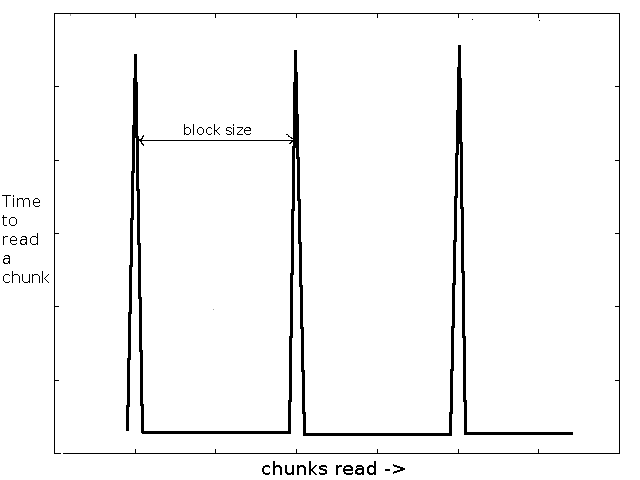
\includegraphics[width=250pt,height=250pt]{buffer_ideal.png}
\begin{center}
Figure 1 : Expected graph for block size experiment.
\end{center}

\subsection{Prefetch}

As mentioned earlier, when the file system detects that the file is being read in a 
sequential manner, it reads the next part of the file before the process issues the read
request. Our approach to measure the amount of prefetching is as follows:
\begin{enumerate}
	\item Read {\tt initial\_portion} bytes sequentially of the file in conveniently sized chunks.
	\item Suspend the process for {\tt duration} seconds.
	\item Read chunks of file sequentially and time the readings.
\end{enumerate}

The initial sequential read is required to trigger the file system's prefetch mechanism.
Suspending the process allows the file system to complete the I/O operations, which might
interfere with our timing measurements later on.

Figure 2 shows the expected graph of the read time measurements. For the data which is
prefetched, the read time is low. As soon as the limit of the prefetch buffer is reached,
there should be a steep increase in the time to read the block, since it involves a disk
access.

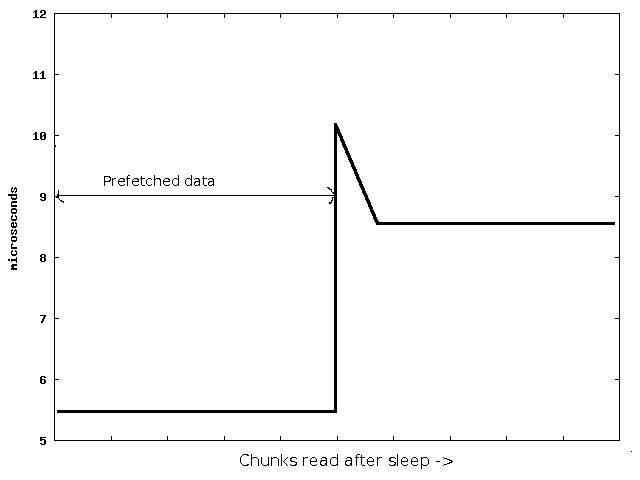
\includegraphics[width=250pt,height=250pt]{prefetch_ideal.png}
\begin{center}
Figure 2 : Expected graph for prefetch experiment.
\end{center}


\subsection{File cache size}

The file system maintains a global file cache, the size of which is limited
dynamically by the Kernel \cite{dynamic_fcache}. The system varies the limit taking into
account current memory utilization and other system load parameters.

This is how we propose measuring the size of the cache:
\begin{enumerate}
	\item Read a file of size {\tt cache\_test\_size} bytes sequentially till the
		 end in conveniently sized chunks.
	\item Read the same file backwards sequentially, until the beginning to the
		file is reached, measuring the time taken for each read.
\end{enumerate}

During the forward read, we will fill the file cache buffers with pages from our
file. If the size of the file is greater than the size of the file cache, then
some of the pages from the beginning of the file are dropped. When we start
reading the file backwards, initially we access pages which are present in the
cache and hence will have low read times. Once we get the pages which were 
dropped from the cache, the read time should shoot up. This allows us to measure
the size of the file cache. Note that this method is unaffected by the page
replacement policy of the cache. Figure 3 illustrates the expected behavior.

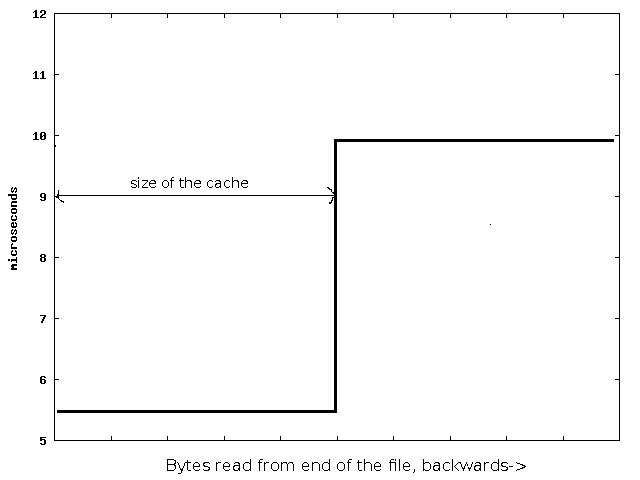
\includegraphics[width=250pt,height=250pt]{cache_ideal.png}
\begin{center}
Figure 3 : Expected graph for cache size test.
\end{center}

This method only works if {\tt cache\_test\_size} is at least as big as the 
file cache, which can be easily ensured by taking it to be some value greater than
the total physical memory on the system.

\subsection{Levels of indirection}
Each inode in the ext2 file system has a number of direct blocks. If the size
of the file grows beyond the size supported by directed blocks, an additional
level of indirection is introduced (more details in \cite{ext2_loi}). We want to determine
the number of direct blocks in the inode. Our approach is as follows:

\begin{enumerate}
	\item Create a new file.
	\item Write chunks of {\tt block\_size} bytes and measure the time taken
		to write.
\end{enumerate}

The expected result is shown in Figure 4. For the first few blocks, the
time to write should be fairly low. But when the size grows beyond the
number of direct blocks, the system has to allocate a block for one
more level of mapping, which would cause a spike in the graph. The writes
after the spike should be slightly higher than the first few writes.

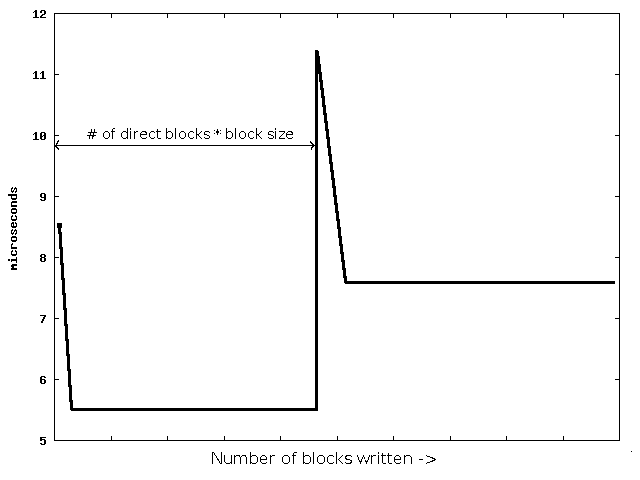
\includegraphics[width=230pt,height=230pt]{indirection_ideal.png}
\begin{center}
Figure 4 : Expected graph for indirection test.
\end{center}


% -------------------------------------------------------------------------
%                               System Details
% -------------------------------------------------------------------------

\section{System Details}
\label{sec:System Details}
\underline{Hardware specifications}: AMD Athlon 64 X2 Dual Core Processor
TK-53 running at 800 MHz, 1 GB DDR2 RAM, Disk TOSHIBA MK8037GS 80 GB
on SATA interface.

\underline{Software specifications}: Linux kernel 2.6.24-16

\underline{Filesystem specifications}: Logical partition size 1.8 GB,
ext2 filesystem.


% -------------------------------------------------------------------------
%                              Results
% -------------------------------------------------------------------------
\section{Implementation and Results}
\label{sec:Implementation and Results}

Each subsection in this section has the following parts:
\begin{enumerate}
	\item Choosing the test parameters: In the test methodology, symbolic
	names are used to denote certain parameters of the test. Specific
	values are given to these parameters in this section.
	\item Source code: A brief and central snippet of the measuring code
	is given. The main logic of the test should be clear from the snippet.
	\item Result: The graph obtained by executing the test is shown in this
	section, along with some information regarding the graph.
	\item Explanation: The graph is compared to the expected graph. Possible
	explanations for some unusual behaviors are also given.
\end{enumerate}

\subsection{Ideal buffer size for random access}

\chumma{Choosing the test parameters}
We use the fact that the ext2 file system allows only blocks of size 1k,4k and 8k
in calculating the parameters mentioned in Section 3.1. We will fix {\tt start\_offset}
to be a random multiple of $LCM(1k,4k,8k) = 8k$, and {\tt quantum} to be 512 bytes.

\chumma{Source code}
\begin{lstlisting}[frame=single]
int start_offset = (rand() % 10 + 1)
   * 8 * KILO_BYTE;

lseek(fd,start_offset,SEEK_SET);

for(int offset = 0;
  offset < 50 * KILO_BYTE;
  offset += quantum ){
  
  u64_t before = rdtsc();
  read(fd,buffer,quantum);
  u64_t after = rdtsc();

  record(offset,
   to_microseconds(before,after));
}
\end{lstlisting}


\chumma{Result}

We repeated the experiment 100 times and took the average of read times.
Figure 5 shows the result we obtained.

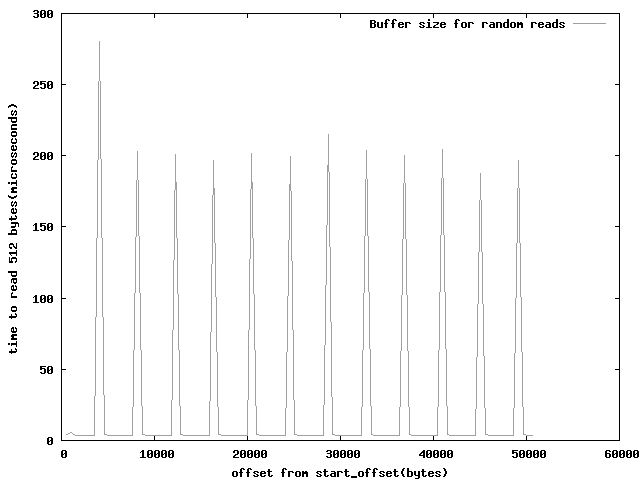
\includegraphics[width=230pt,height=230pt]{buffer_size.png}
\begin{center}
Figure 5 : Measured graph for block size test.
\end{center}


\chumma{Explanation}
The graph is as expected. There is a periodic spike at every 8$^{th}$
measurement, which indicates a block size of 4k. The in-memory read
takes around 5-6 \mus on average, whereas a read which accesses
the disk takes around 200 \mus, which is too low if the disk
had to seek and read the platter, which indicates that the disk actually
reads more than one block at a time.

\subsection{Prefetch}

\chumma{Choosing the test parameters}
We need to choose {\tt initial\_portion} large enough to trigger the
prefetch mechanism of the kernel. In our tests, we use 1M, 2M, 4M and
8M as possible values for this variable. The {\tt duration} parameter
should be large enough to allow the prefetch to complete. We err on the
side on caution and wait for 1 second before we start measuring.

\chumma{Source code}
\begin{lstlisting}[frame=single]
//initial read
while( size < initial_portion ){
  read(file,buffer,buffer_size);
  size += buffer_size;
}

//wait for a second
sleep(1);
size = 0;

//time the reads
while(size < MEGA_BYTE ){
  u64_t before = rdtsc();
  read(file,buffer,buffer_size);
  u64_t after  = rdtsc();
  record(size,
    to_microseconds(before,after));
  size += ret;
}
\end{lstlisting}

\chumma{Result}

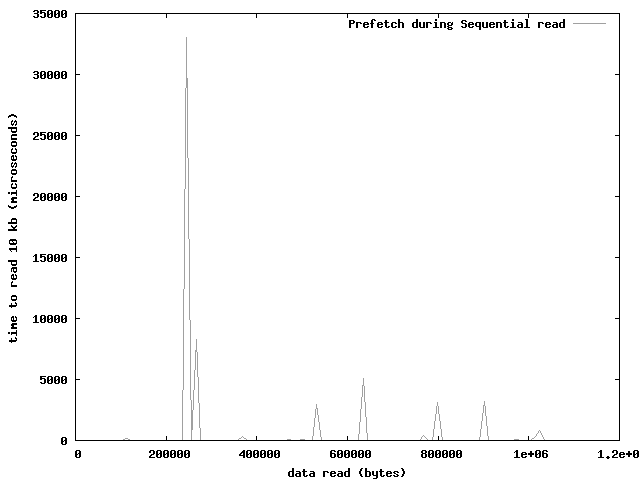
\includegraphics[width=250pt,height=250pt]{prefetch.png}
\begin{center}
Figure 6 : Measured graph for prefetch test.
\end{center}

The graph shown in Figure 6 shows the measurements for {\tt start\_offset}
set to 1 MB.

\chumma{Explanation}

 The plots of the different measurements are approximately
the same, which shows that {\tt start\_offset} doesn't have a great impact on
the amount that is prefetched. We see that the first and largest spike occurs
at around 240k which gives us the amount that is prefetched. The average value
of the spike is around 35000 \mus which indicates that the read call did actually
go to the disk and fetch the data.

\subsection{File cache size}

\chumma{Choosing the test parameters}

The size of the input file needs to be larger than the amount of physical memory
available, which is 1GB, so that is the size of the file chosen.

\chumma{Source code}
\begin{lstlisting}[frame=single]
//initial forward read of the file
while(true){
  ret = read(fd,buffer,buffer_size);
  if(ret <= 0) break;
  size += ret;
}

//backward timed read of the file
while(size > MEGA_BYTE){
  lseek(fd,-buffer_size,SEEK_CUR);
  
  u64_t before = rdtsc();
  read(fd,buffer,buffer_size);
  u64_t after = rdtsc();

  record(size,
   to_microseconds(before,after) );

  lseek(fd,-buffer_size,SEEK_CUR);
  size -= buffer_size;
}
\end{lstlisting}

\chumma{Result}

The experiment was repeated 5 times, and the average of the
measurements is plotted in graph 7. Between each repetition of
the experiment, the global file cache was cleared using the
following Linux command \cite{drop_cache}:

{\tt echo 3 > /proc/sys/vm/drop\_cache}

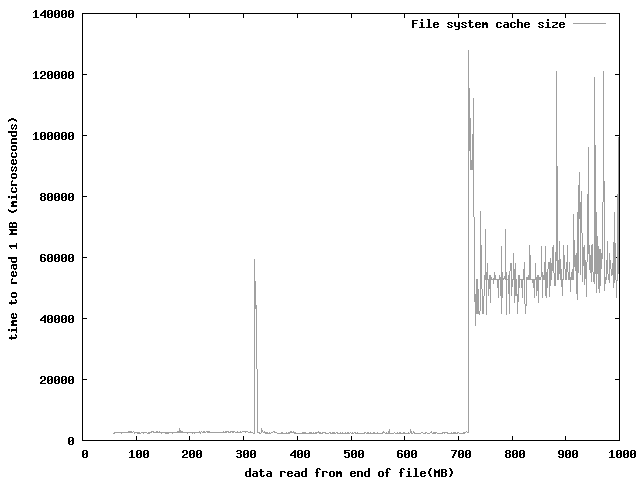
\includegraphics[width=250pt,height=250pt]{cache_size.png}
\begin{center}
Figure 7 : Measured graph for cache size test.
\end{center}

\chumma{Explanation}

The result graph is also as expected. For the first 709 megabytes,
the read times are very low, of the order of 2000 \mus / read. This
clearly indicates that the disk is not being accessed. There is a
steep climb in the read time after 709 MB, with read time averaging
around 60000 \mus / read, which indicates that the data is no longer
fetched from the cache.

\subsection{Levels of indirection}

\chumma{Choosing the test parameters}
From the first experiment, we can fix the {\tt block\_size} to be 4k.

\chumma{Source code}
\begin{lstlisting}[frame=single]
size = 0;
while(size < 100 * KILO_BYTE){

  u64_t before = rdtsc();
  write(fd,buffer,4 * KILO_BYTE);
  //this is important
  fsync(fd);
  u64_t after = rdtsc();
  
  record(size,
   to_microseconds(before,after));
  size += 4 * KILO_BYTE;
}
\end{lstlisting}

\chumma{Result}

The experiment was repeated 10 times, and the average write times
were used. The resultant graph is shown in Figure 8.

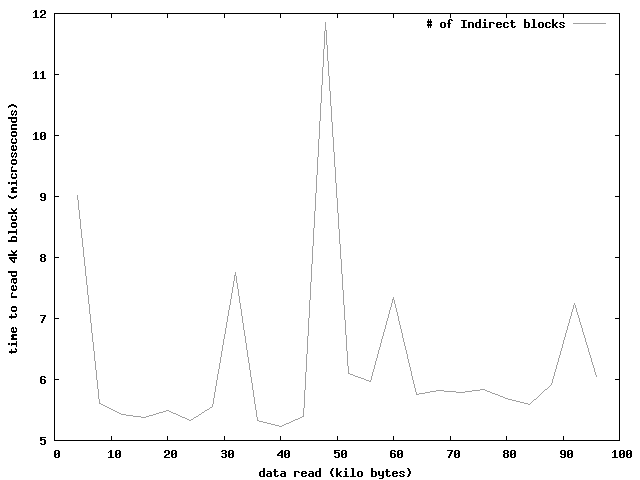
\includegraphics[width=230pt,height=230pt]{indirection.png}
\begin{center}
Figure 8 : Measured graph for indirection test.
\end{center}

\chumma{Explanation}

The graph is as expected. There is a significant spike at 48k which
is consistent with the number of blocks being 12. Apart from the main
spike, there are a few more smaller spikes. The first spike is caused
the system initially allocating a group of blocks. Since there is another
spike at block 8, we can deduce that the file system allocates 7 blocks
at the time of file creation. At block 8, the spike indicates that the
system allocates 4 more blocks. At block 12, the spike indicates that the
direct blocks are all allocated, so a level of indirection has to be
introduced.

% -------------------------------------------------------------------------
%                              Conclusions
% -------------------------------------------------------------------------
\section{Conclusions}
\label{sec:Conclusions}

The results of our tests are summarized in the following table.

\begin{tabular}{|c|l|}
\hline
	\textbf{Property} & \textbf{Measured Value} \\
\hline
	Block Size & 4 KB \\
\hline
	Prefetch Size & 239 KB \\
\hline
	Cache Size & 709 MB \\
\hline
	\# of direct blocks & 12 \\
\hline
\end{tabular}


Overall, the results obtained by the experiment agree well with the expected
outcome. The results regarding cache size must be taken with a pinch of salt,
since the system dynamically manages the size of the cache, the experiment
is not perfectly reproducible. The effect of the hard disk cache, which is
quite large in modern disks (2 MB-8 MB), is also something which is not handled
by our prefetch test, which might affect the prefetch value.
\end{sloppypar}
% -------------------------------------------------------------------------
%                             End Stuff
% -------------------------------------------------------------------------

\setlength{\baselineskip}{12pt}

\noindent{
\bibliography{cs736-miniproject-report}
\bibliographystyle{abbrvurl3}
}

\end{document}
